% Member E's report sections (advanced studies, Discussion, Conclusion), for pasting into the
% team's Overleaf project. Written by Johnnie Parris, who took over Member E's share.
% References: docs/refs/member_e.bib (plus zuiderveld1994clahe from method1.bib).
% Figures: docs/report/figures/e_*.pdf, made by scripts/make_e_figures.py.
% Every number is on the TEST split unless stated, from a committed CSV named in a comment
% beside it. Thresholds for P/R/count are each method's best-F1 threshold on clean val.
% Budget (PROJECT_PLAN.md section 7): ~0.4 p Methods, ~1 p Results, ~1.5 p Discussion, 0.5 p Conclusion.

% ---------------------------------------------------------------------------------------------
% In Section 3, Methods
% ---------------------------------------------------------------------------------------------
\subsection{Advanced Studies}
\label{sec:advanced}

\textbf{Robustness.} Following Hendrycks and Dietterich~\cite{hendrycks2019benchmarking} and its
detection counterpart~\cite{michaelis2019benchmarking}, we built distorted copies of the val and
test splits with five corruptions at three severities: Gaussian noise ($\sigma=10,25,50$ on
0--255), Gaussian blur ($\sigma=1,2,4$\,px), low light ($I'=a(I-\mu)+a\mu$ with $a=0.6,0.4,0.2$,
which lowers contrast and brightness together), JPEG compression (quality 30, 15, 5) and
occlusion (a grey rectangle covering 25, 50 or 75\% of every bird box). Each random draw is
seeded from the image name, so the 15 variants are reproducible. Labels are unchanged. Every
method was run once per variant on test; val variants were used only to tune mitigations.
For Methods~1 and~2 the mitigation is one global preprocessing step, chosen from nine
combinations of median, bilateral~\cite{tomasi1998bilateral} or non-local-means~\cite{buades2005nonlocal}
denoising and CLAHE~\cite{zuiderveld1994clahe} by the mean val mAP@0.5 of Method~1 over the
clean and 15 distorted val sets. A per-distortion choice would assume the corruption is known
at test time. Method~2's classifier is retrained on preprocessed images. For YOLO the mitigation
is training-time distortion augmentation: each training image is replaced, with probability 0.5,
by a randomly chosen corruption and severity.

\textbf{Data and label efficiency.} YOLO11n~\cite{ultralytics2024yolo11} was retrained from COCO
weights on nested random subsets of 10, 25 and 50\% of the training images, on all images with
every box edge jittered by up to $\pm$20\% of the box size, and on all images with 20\% of boxes
deleted. All runs share the tuned optimiser and loss settings and Ultralytics' default online
augmentation (mosaic, flips, HSV, scale). Full-data runs train for 30 epochs; a subset of
fraction $f$ trains for $\min(30/f, 100)$ epochs so that the smaller sets are not also
under-trained. As an improvement for the low-data regime we add stronger augmentation to the
10\% run (heavier mosaic, scale and colour jitter, mixup and copy-paste~\cite{ghiasi2021copypaste}).
Each run's checkpoint is the epoch with the best clean val mAP@0.5, and is evaluated once on test.

\textbf{Density and failure analysis.} Test images are binned by bird count (0, 1--10, 11--50,
51--100; no test image has more than 100 birds), and birds by box width into equal thirds. Each
error is assigned automatically to one of five types: a miss inside a flock (at least three
other birds within two box diagonals), an isolated miss, a duplicate detection, a poorly
localised box ($0.1\le$ IoU $<0.5$) and a background false alarm (IoU $<0.1$).

% ---------------------------------------------------------------------------------------------
% In Section 4, Experimental Results
% ---------------------------------------------------------------------------------------------
\subsection{Robustness to Image Distortions}
\label{sec:res-robust}

% Numbers: results/robustness_test.csv (mAP50 per method x variant, test split).
Fig.~\ref{fig:robust} and Table~\ref{tab:robust} show how test mAP@0.5 changes under the five
corruptions. The learned detectors stay far ahead in absolute terms: averaged over all 15
distorted sets, YOLO reaches 0.535 and Faster R-CNN 0.524, against 0.082 for Method~2 and 0.040
for Method~1. In relative terms, however, they lose more. YOLO keeps 64\% of its clean mAP on
average and Faster R-CNN 63\%, while Method~1 keeps 86\%, mostly because its clean score is
already near the floor.

Mild corruptions barely matter: at severity~1 every detector stays within 10\% of its clean
score, except under occlusion. The damage comes at the top severities, and the two detectors
fail differently. Strong noise ($\sigma=50$) cuts YOLO to 0.215 but Faster R-CNN only to 0.418,
whereas heavy blur ($\sigma=4$\,px) hurts both about equally (0.341 and 0.300), as does JPEG
quality~5 (0.182 and 0.183). Low light is the most benign corruption: at a fifth of the original
contrast YOLO still scores 0.709. Occlusion is the worst. Covering a quarter of each bird drops
YOLO to 0.506; covering three quarters leaves it at 0.014, and Method~2 at zero. Method~1 falls
to about 0.02 at every occlusion level, since the grey patch breaks the colour contrast its
segmentation relies on.

\begin{table}[t]
\centering
\caption{Share of clean test mAP@0.5 kept under each corruption (mean over the three
severities). ``+dn'' adds the denoising chosen on val.}
\label{tab:robust}
\setlength{\tabcolsep}{3.5pt}
\begin{tabular}{lcccccc}
\hline
 & M1 & M1+dn & M2 & M2+dn & YOLO & F-RCNN \\
\hline
Clean mAP@0.5 & 0.047 & 0.051 & 0.116 & 0.123 & 0.832 & 0.825 \\
Noise     & 0.98 & 0.87 & 0.83 & 0.78 & 0.65 & 0.76 \\
Blur      & 1.07 & 0.98 & 0.90 & 0.81 & 0.75 & 0.70 \\
Low light & 0.92 & 0.86 & 0.89 & 0.85 & 0.93 & 0.86 \\
JPEG      & 0.89 & 0.90 & 0.84 & 0.86 & 0.64 & 0.66 \\
Occlusion & 0.44 & 0.42 & 0.09 & 0.08 & 0.25 & 0.20 \\
\hline
\end{tabular}
\end{table}

\begin{figure*}[t]
\centering
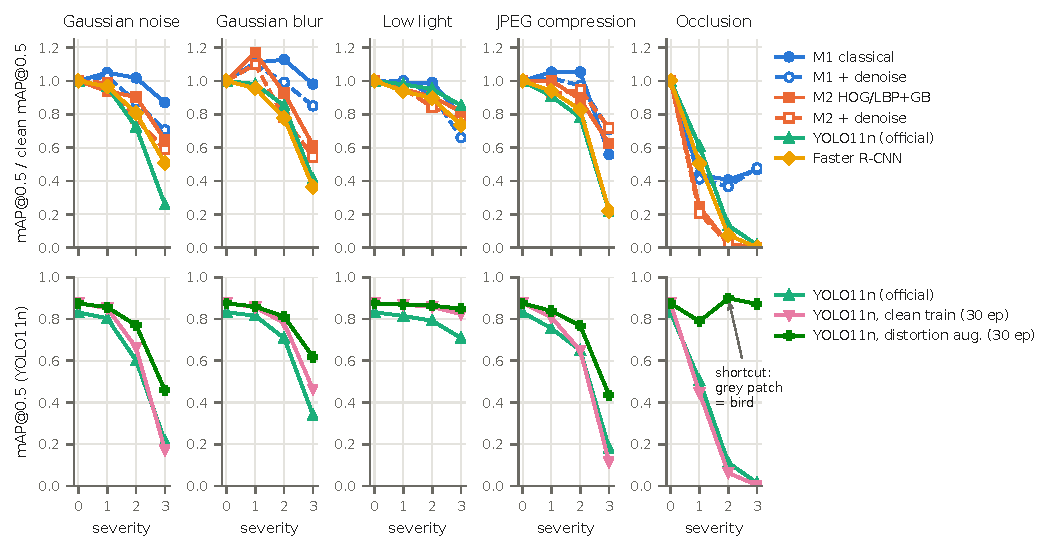
\includegraphics[width=\textwidth]{figures/e_robustness.pdf}
\caption{Robustness on the test set. Top: mAP@0.5 relative to each method's clean score;
dashed lines add the val-selected denoising. Bottom: absolute mAP@0.5 of YOLO11n, comparing the
team's model with our 30-epoch retraining with and without distortion augmentation.}
\label{fig:robust}
\end{figure*}

\textbf{Mitigation.} For the classical methods, CLAHE lowered val mAP under every corruption
(Method~1 clean val: 0.102 without, 0.055 with), because it changes the colour contrast that
the segmentation thresholds were tuned on. The val-selected setting is therefore light
non-local-means denoising alone ($h=5$), whose mean val mAP over the 16 val sets was 0.0786
against 0.0777 with no preprocessing. On test it helps where compression artefacts dominate (JPEG
quality~5: Method~1 0.026$\rightarrow$0.036, Method~2 0.072$\rightarrow$0.088) and raises the
clean scores slightly, but the average over all distorted sets is unchanged (0.040$\rightarrow$0.041
and 0.082$\rightarrow$0.083). Preprocessing cannot restore birds that the corruption has removed.
% ROBUST-AUG: fill from results/robustness_test.csv rows e_de_100 / e_robust_aug.

\subsection{Data and Label Efficiency}
\label{sec:res-data}

% FILL: results/data_efficiency_test.csv

% ---------------------------------------------------------------------------------------------
% Section 5, Discussion
% ---------------------------------------------------------------------------------------------
\section{Discussion}
\label{sec:discussion}

% Clean test numbers: analysis/summary.csv (python src/analysis.py), thresholds from val.
% Density/size: analysis/density_bins.csv, analysis/size_bins.csv. Errors: results/failure_categories_test.csv.
% Timing: results/ml_test_comparison.csv (YOLO, Faster R-CNN; CPU, this Mac), results/m1_test.meta.json,
% src/ml/README.md (M2). Training: results/timelines/*.csv (CUDA), results/e_runs (MPS).

\textbf{Why the learned detectors win.} YOLO11n (0.832 mAP@0.5) and Faster R-CNN (0.825) are
an order of magnitude ahead of Method~2 (0.116) and Method~1 (0.047). The failure breakdown in
Fig.~\ref{fig:failures} shows why. Both classical methods miss most birds (recall 0.10 and
0.16), and about two thirds of those misses are birds inside flocks: segmentation merges
touching birds into one component, which the shape filter then rejects or boxes as one bird.
Method~2 can only rescore Method~1's candidates, so it inherits those misses. The CNNs learn
multi-scale features that separate neighbouring birds, which cuts flock misses from 921
(Method~1) to 217 (YOLO), and they learn what is \emph{not} a bird. Background false alarms on
the 27 empty test images fall from 2.7 per image for both classical methods to 0.19 (YOLO) and
0.26 (Faster R-CNN). The two CNNs make similar numbers of errors (582 and 586), but of
different kinds. Faster R-CNN misses fewer isolated birds (101 vs 128) but produces more
duplicate boxes in flocks (70 vs 47) and misses more birds in the two densest test images
(recall 0.46 vs 0.59).

\textbf{Density and size.} Every method degrades with crowding (Fig.~\ref{fig:density}). YOLO's
mAP falls from 0.886 on images with 1--10 birds to 0.814 at 11--50 and 0.680 at 51--100, and
its counting error grows from 0.5 to 14.5 birds per image. Small birds are the main reason:
YOLO finds 61\% of the smallest third of birds (narrower than 6.3\% of the image) but 89\%
of the largest, and Faster R-CNN 57\% and 93\%. The test split contains only two images with
more than 50 birds and none above 100 (only two training images exceed 100), so the
high-density results rest on very few images.

\textbf{Speed and accuracy.} On one Apple M5 Pro CPU, Method~1 needs 4.9\,ms per image with no
training, Method~2 about 70\,ms after about 100\,s of training, YOLO11n 56\,ms and Faster R-CNN
451\,ms. Training took 46\,min for YOLO and 55\,min for Faster R-CNN on a CUDA GPU. YOLO is
therefore both the most accurate and, among the learned methods, the fastest: eight times
faster than Faster R-CNN for equal accuracy. Method~1 remains useful only where speed or the
absence of training data matter more than recall.

\textbf{What the studies show.} Robustness and accuracy are different properties. The CNNs lose
a larger share of their score under corruption than the classical methods, because they exploit
fine texture that noise, blur and compression destroy, while the classical methods have little
to lose. Faster R-CNN is clearly more tolerant of noise than YOLO, plausibly because its much
larger ResNet-50 backbone averages out pixel noise better than YOLO11n's small backbone at the
same 640-pixel input. Occlusion is the hardest case for all: detectors that recognise birds by
their whole silhouette fail when half of it is hidden, which is what happens inside dense
flocks too. Simple preprocessing does not fix this; the corruption has to be seen in training.
% DE-DISCUSSION: fill from results/data_efficiency_test.csv.

\begin{figure}[t]
\centering
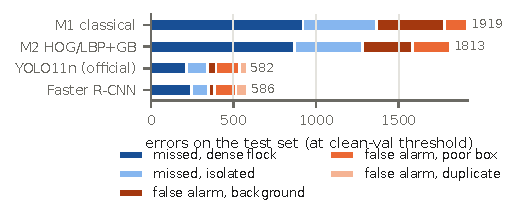
\includegraphics[width=\columnwidth]{figures/e_failures.pdf}
\caption{Test-set errors by type at each method's val-selected threshold.}
\label{fig:failures}
\end{figure}

\begin{figure*}[t]
\centering
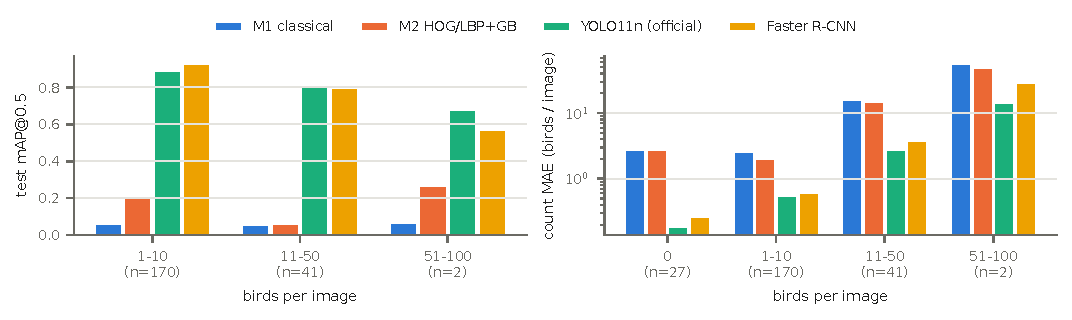
\includegraphics[width=\textwidth]{figures/e_density.pdf}
\caption{Test mAP@0.5 and counting error by number of birds per image ($n$ = images per bin).
Count MAE uses a log scale.}
\label{fig:density}
\end{figure*}

\begin{figure*}[t]
\centering
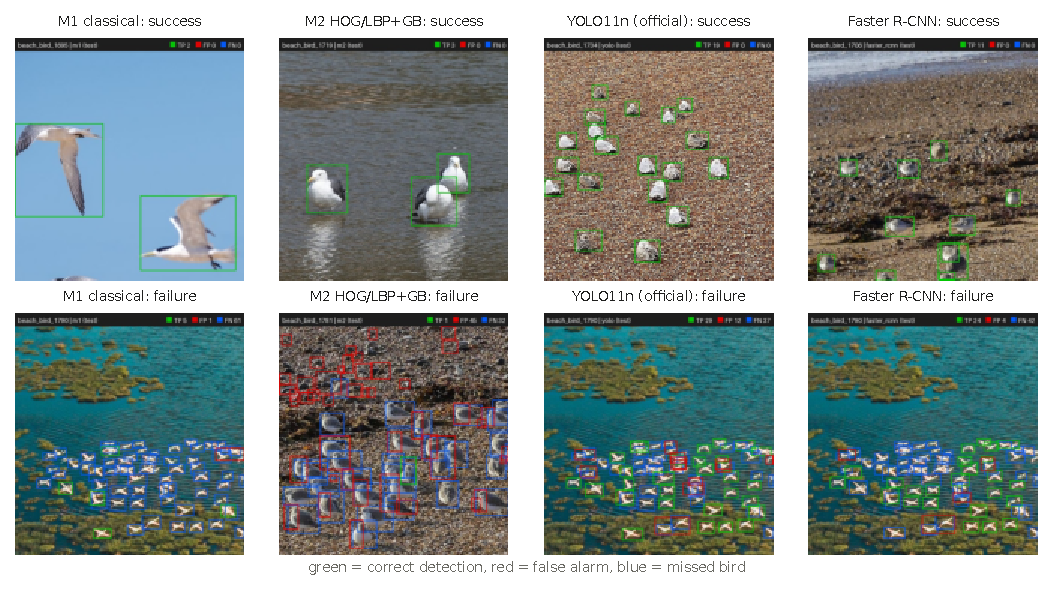
\includegraphics[width=\textwidth]{figures/e_gallery.pdf}
\caption{Best (top) and worst (bottom) test images for each method. Green: correct detection;
red: false alarm; blue: missed bird.}
\label{fig:gallery}
\end{figure*}

% ---------------------------------------------------------------------------------------------
% Section 6, Conclusion
% ---------------------------------------------------------------------------------------------
\section{Conclusion}
\label{sec:conclusion}

% FILL
